% Options for packages loaded elsewhere
\PassOptionsToPackage{unicode}{hyperref}
\PassOptionsToPackage{hyphens}{url}
%
\documentclass[
]{article}
\usepackage{amsmath,amssymb}
\usepackage{lmodern}
\usepackage{iftex}
\ifPDFTeX
  \usepackage[T1]{fontenc}
  \usepackage[utf8]{inputenc}
  \usepackage{textcomp} % provide euro and other symbols
\else % if luatex or xetex
  \usepackage{unicode-math}
  \defaultfontfeatures{Scale=MatchLowercase}
  \defaultfontfeatures[\rmfamily]{Ligatures=TeX,Scale=1}
\fi
% Use upquote if available, for straight quotes in verbatim environments
\IfFileExists{upquote.sty}{\usepackage{upquote}}{}
\IfFileExists{microtype.sty}{% use microtype if available
  \usepackage[]{microtype}
  \UseMicrotypeSet[protrusion]{basicmath} % disable protrusion for tt fonts
}{}
\makeatletter
\@ifundefined{KOMAClassName}{% if non-KOMA class
  \IfFileExists{parskip.sty}{%
    \usepackage{parskip}
  }{% else
    \setlength{\parindent}{0pt}
    \setlength{\parskip}{6pt plus 2pt minus 1pt}}
}{% if KOMA class
  \KOMAoptions{parskip=half}}
\makeatother
\usepackage{xcolor}
\usepackage[margin=1in]{geometry}
\usepackage{color}
\usepackage{fancyvrb}
\newcommand{\VerbBar}{|}
\newcommand{\VERB}{\Verb[commandchars=\\\{\}]}
\DefineVerbatimEnvironment{Highlighting}{Verbatim}{commandchars=\\\{\}}
% Add ',fontsize=\small' for more characters per line
\usepackage{framed}
\definecolor{shadecolor}{RGB}{248,248,248}
\newenvironment{Shaded}{\begin{snugshade}}{\end{snugshade}}
\newcommand{\AlertTok}[1]{\textcolor[rgb]{0.94,0.16,0.16}{#1}}
\newcommand{\AnnotationTok}[1]{\textcolor[rgb]{0.56,0.35,0.01}{\textbf{\textit{#1}}}}
\newcommand{\AttributeTok}[1]{\textcolor[rgb]{0.77,0.63,0.00}{#1}}
\newcommand{\BaseNTok}[1]{\textcolor[rgb]{0.00,0.00,0.81}{#1}}
\newcommand{\BuiltInTok}[1]{#1}
\newcommand{\CharTok}[1]{\textcolor[rgb]{0.31,0.60,0.02}{#1}}
\newcommand{\CommentTok}[1]{\textcolor[rgb]{0.56,0.35,0.01}{\textit{#1}}}
\newcommand{\CommentVarTok}[1]{\textcolor[rgb]{0.56,0.35,0.01}{\textbf{\textit{#1}}}}
\newcommand{\ConstantTok}[1]{\textcolor[rgb]{0.00,0.00,0.00}{#1}}
\newcommand{\ControlFlowTok}[1]{\textcolor[rgb]{0.13,0.29,0.53}{\textbf{#1}}}
\newcommand{\DataTypeTok}[1]{\textcolor[rgb]{0.13,0.29,0.53}{#1}}
\newcommand{\DecValTok}[1]{\textcolor[rgb]{0.00,0.00,0.81}{#1}}
\newcommand{\DocumentationTok}[1]{\textcolor[rgb]{0.56,0.35,0.01}{\textbf{\textit{#1}}}}
\newcommand{\ErrorTok}[1]{\textcolor[rgb]{0.64,0.00,0.00}{\textbf{#1}}}
\newcommand{\ExtensionTok}[1]{#1}
\newcommand{\FloatTok}[1]{\textcolor[rgb]{0.00,0.00,0.81}{#1}}
\newcommand{\FunctionTok}[1]{\textcolor[rgb]{0.00,0.00,0.00}{#1}}
\newcommand{\ImportTok}[1]{#1}
\newcommand{\InformationTok}[1]{\textcolor[rgb]{0.56,0.35,0.01}{\textbf{\textit{#1}}}}
\newcommand{\KeywordTok}[1]{\textcolor[rgb]{0.13,0.29,0.53}{\textbf{#1}}}
\newcommand{\NormalTok}[1]{#1}
\newcommand{\OperatorTok}[1]{\textcolor[rgb]{0.81,0.36,0.00}{\textbf{#1}}}
\newcommand{\OtherTok}[1]{\textcolor[rgb]{0.56,0.35,0.01}{#1}}
\newcommand{\PreprocessorTok}[1]{\textcolor[rgb]{0.56,0.35,0.01}{\textit{#1}}}
\newcommand{\RegionMarkerTok}[1]{#1}
\newcommand{\SpecialCharTok}[1]{\textcolor[rgb]{0.00,0.00,0.00}{#1}}
\newcommand{\SpecialStringTok}[1]{\textcolor[rgb]{0.31,0.60,0.02}{#1}}
\newcommand{\StringTok}[1]{\textcolor[rgb]{0.31,0.60,0.02}{#1}}
\newcommand{\VariableTok}[1]{\textcolor[rgb]{0.00,0.00,0.00}{#1}}
\newcommand{\VerbatimStringTok}[1]{\textcolor[rgb]{0.31,0.60,0.02}{#1}}
\newcommand{\WarningTok}[1]{\textcolor[rgb]{0.56,0.35,0.01}{\textbf{\textit{#1}}}}
\usepackage{graphicx}
\makeatletter
\def\maxwidth{\ifdim\Gin@nat@width>\linewidth\linewidth\else\Gin@nat@width\fi}
\def\maxheight{\ifdim\Gin@nat@height>\textheight\textheight\else\Gin@nat@height\fi}
\makeatother
% Scale images if necessary, so that they will not overflow the page
% margins by default, and it is still possible to overwrite the defaults
% using explicit options in \includegraphics[width, height, ...]{}
\setkeys{Gin}{width=\maxwidth,height=\maxheight,keepaspectratio}
% Set default figure placement to htbp
\makeatletter
\def\fps@figure{htbp}
\makeatother
\setlength{\emergencystretch}{3em} % prevent overfull lines
\providecommand{\tightlist}{%
  \setlength{\itemsep}{0pt}\setlength{\parskip}{0pt}}
\setcounter{secnumdepth}{-\maxdimen} % remove section numbering
\ifLuaTeX
  \usepackage{selnolig}  % disable illegal ligatures
\fi
\IfFileExists{bookmark.sty}{\usepackage{bookmark}}{\usepackage{hyperref}}
\IfFileExists{xurl.sty}{\usepackage{xurl}}{} % add URL line breaks if available
\urlstyle{same} % disable monospaced font for URLs
\hypersetup{
  pdftitle={Quantitative Analysis in Ecology and Evolution},
  pdfauthor={Øystein H. Opedal},
  hidelinks,
  pdfcreator={LaTeX via pandoc}}

\title{Quantitative Analysis in Ecology and Evolution}
\usepackage{etoolbox}
\makeatletter
\providecommand{\subtitle}[1]{% add subtitle to \maketitle
  \apptocmd{\@title}{\par {\large #1 \par}}{}{}
}
\makeatother
\subtitle{The Linear Model 1: Linear regression}
\author{Øystein H. Opedal}
\date{19 Oct 2022}

\begin{document}
\maketitle

\hypertarget{the-linear-model-i-introduction-and-linear-regression}{%
\subsection{4. The linear model I: Introduction and linear
regression}\label{the-linear-model-i-introduction-and-linear-regression}}

Nearly all the statistical models we will discuss in this text are forms
of the linear model

\(y_i = \beta_0 + \Sigma_j x_{ij} \beta_j + \epsilon_i\)

The term \(\beta_0\) (sometimes denoted \(\alpha\)) is the
\emph{intercept}, which in the context of a linear regression gives the
value of the response variable \(y\) when the predictor variable \(x\)
is zero. The \(\beta_j\) are the coefficients (`slopes') for the
predictor variables \(x\), and the \(\epsilon\) represent the
\emph{residuals}, the deviations of each data point from it's expected
value based on the fitted model. In a regression, the residual is the
perpendicular distance from the fitted regression line to each data
point. The linear model assumes that the residuals (not the data!) are
normally distributed, though minor deviations from this is not generally
a problem.

In the following, we will consider a series of examples of linear models
fitted to simulated data. After simulating some values of the predictor
\(x\), we define \(y\) as a function of \(x\) and add some residual
variance to the data (i.e.~we simulate data from the same linear model
that we will eventually fit to the data.) The advantage of starting from
simulated data is that we know the true values of the parameters we will
try to estimate. This is very useful when we want to check that our
analysis is doing what we think it is doing.

As noted above, \texttt{R} functions know the order of arguments. Note
how the second incidence of \texttt{rnorm} below skips the formalities.

\begin{Shaded}
\begin{Highlighting}[]
\FunctionTok{set.seed}\NormalTok{(}\DecValTok{85}\NormalTok{)}
\NormalTok{x }\OtherTok{=} \FunctionTok{rnorm}\NormalTok{(}\AttributeTok{n=}\DecValTok{200}\NormalTok{, }\AttributeTok{mean=}\DecValTok{10}\NormalTok{, }\AttributeTok{sd=}\DecValTok{2}\NormalTok{)}
\NormalTok{y }\OtherTok{=} \FloatTok{0.4}\SpecialCharTok{*}\NormalTok{x }\SpecialCharTok{+} \FunctionTok{rnorm}\NormalTok{(}\DecValTok{200}\NormalTok{, }\DecValTok{0}\NormalTok{, }\DecValTok{1}\NormalTok{)}

\FunctionTok{plot}\NormalTok{(x, y, }\AttributeTok{las=}\DecValTok{1}\NormalTok{, }
     \AttributeTok{xlab=}\StringTok{"Leaf length (mm)"}\NormalTok{, }
     \AttributeTok{ylab=}\StringTok{"Leaf width (mm)"}\NormalTok{)}
\end{Highlighting}
\end{Shaded}

\includegraphics{Chapter2_LinReg_files/figure-latex/unnamed-chunk-1-1.pdf}

At this point let's talk about how to write \texttt{R} code. In the
\texttt{R} chunks above you may start to notice some `style
conventions'. When we are new to \texttt{R} and coding, most of us write
really messy code. It is now becoming mandatory to publish our code
alongside our papers, and we thus have to learn to write code that is
easy to read and pleasent to look at. I don't follow all the `rules'
around this, but at least I try to be consistent. For example, the
strict \texttt{R} convention has been to use the \texttt{\textless{}-}
operator for assignments, but I find the \texttt{=} easier. Note though
the spaces to either side of \texttt{=} that makes the code easier to
read. Within functions, add a space after commas.

In scatterplots, a useful change from the default is to make the
\emph{y}-axis labels horizontal by setting \texttt{las=1}. There are
hundreds of ways to change the appearence of \texttt{R}-plots, see the
wonderful world of \texttt{par()}. If you prefer, you can choose to
learn alternative plotting frameworks such as \texttt{ggplot}, but these
lecture notes will use \texttt{R} packages only when strictly needed.

The aim of regression analysis is to estimate the linear relationship
between a response variable (or `dependent variable') and one or more
predictor variables (`independent variables'). The most common form of
regression analysis is so-called ordinary least-square (OLS) regression,
in which the regression parameters are estimated so as to minimize the
square deviations of the data points from the estimated regression line.
The deviations are termed \emph{residuals}, and are assumed to be
normally distributed.

\begin{Shaded}
\begin{Highlighting}[]
\NormalTok{m }\OtherTok{=} \FunctionTok{lm}\NormalTok{(y}\SpecialCharTok{\textasciitilde{}}\NormalTok{x)}
\end{Highlighting}
\end{Shaded}

The object \texttt{m} now holds the fitted model. Let's extract the
model coefficients and produce some plots of the residuals.

\begin{Shaded}
\begin{Highlighting}[]
\NormalTok{cf }\OtherTok{=} \FunctionTok{summary}\NormalTok{(m)}\SpecialCharTok{$}\NormalTok{coef}
\NormalTok{predvals }\OtherTok{=}\NormalTok{ cf[}\DecValTok{1}\NormalTok{,}\DecValTok{1}\NormalTok{] }\SpecialCharTok{+}\NormalTok{ cf[}\DecValTok{2}\NormalTok{,}\DecValTok{1}\NormalTok{]}\SpecialCharTok{*}\NormalTok{x}

\FunctionTok{par}\NormalTok{(}\AttributeTok{mfrow=}\FunctionTok{c}\NormalTok{(}\DecValTok{1}\NormalTok{,}\DecValTok{2}\NormalTok{))}
\FunctionTok{plot}\NormalTok{(x, y, }\AttributeTok{las=}\DecValTok{1}\NormalTok{)}
\FunctionTok{abline}\NormalTok{(m)}
\FunctionTok{segments}\NormalTok{(x, y, x, predvals)}
\FunctionTok{hist}\NormalTok{(}\FunctionTok{residuals}\NormalTok{(m), }\AttributeTok{las=}\DecValTok{1}\NormalTok{)}
\end{Highlighting}
\end{Shaded}

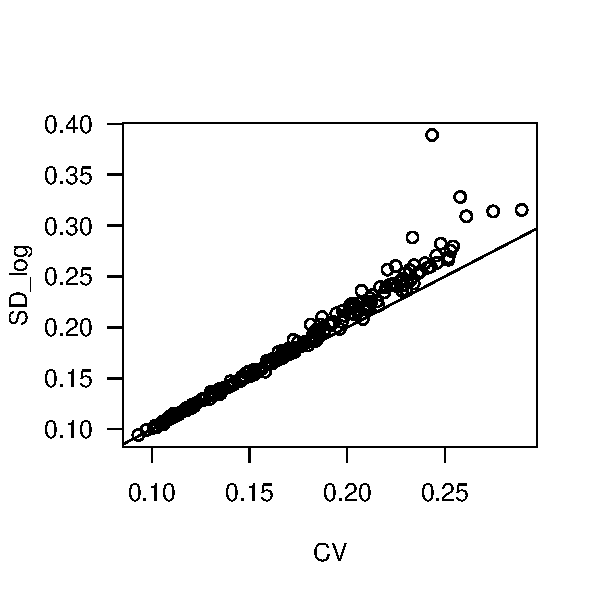
\includegraphics{Chapter2_LinReg_files/figure-latex/unnamed-chunk-3-1.pdf}

These residuals are fine, as is of course fully expected given that we
simulated the data from the (gaussian) linear model. There are many
other ways of assessing whether the model assumptions are met, see for
example what happens if you call \texttt{plot(m)} after setting
\texttt{par(mfrow=c(2,2))}. Notice that the \texttt{plot} function is
\emph{generic}, it produces a different result depending on what is fed
to it. If we call \texttt{plot(x,y)} when both \texttt{x} and \texttt{y}
are continuous variables, we get a scatterplot. If \texttt{x} is a
factor, we get a boxplot.

Let's now have a look at the results of our linear model fit.

\begin{Shaded}
\begin{Highlighting}[]
\FunctionTok{summary}\NormalTok{(m)}
\end{Highlighting}
\end{Shaded}

\begin{verbatim}
## 
## Call:
## lm(formula = y ~ x)
## 
## Residuals:
##      Min       1Q   Median       3Q      Max 
## -2.45122 -0.68319  0.02913  0.69861  2.88937 
## 
## Coefficients:
##             Estimate Std. Error t value Pr(>|t|)    
## (Intercept) -0.40114    0.35186   -1.14    0.256    
## x            0.43330    0.03538   12.25   <2e-16 ***
## ---
## Signif. codes:  0 '***' 0.001 '**' 0.01 '*' 0.05 '.' 0.1 ' ' 1
## 
## Residual standard error: 0.9912 on 198 degrees of freedom
## Multiple R-squared:  0.4311, Adjusted R-squared:  0.4282 
## F-statistic:   150 on 1 and 198 DF,  p-value: < 2.2e-16
\end{verbatim}

This summary contains a lot of information. First, we can see some
quantiles of the residual distribution, which confirms what we have
already seen from the histogram: the residuals are fine because the
median is close to zero, the 1st and 3rd quartile are symmetrical, and
the min and max values are nearly symmetrical too.

Next we see the model parameter estimates, their standard errors, a test
statistic (\(t\)), and a \(P\)-value. It is tempting to look first at
the \(P\)-value, the magic measure of significance and, to some,
`importance'. Before going on, let's take a moment to recall what the
\(P\)-value means and how it is obtained. In the context of the linear
regression above, the test statistic \(t\) is given by
\(t = \frac{\hat{\beta}}{SE(\beta)}\). We already know that the standard
error \(SE=\frac{\sigma}{\sqrt{n}}\), thus

\(t = \frac{\hat{\beta}}{\frac{\sigma(\hat{\beta})}{\sqrt{n}}}\)

The most important thing to notice here is that the sample size \(n\) is
in the denominator of the expression for the standard error, so that
larger sample size will lead to a smaller standard error, and thus a
greater \(t\)-value.

The \(P\)-value is the probability of observing the observed value of
the test statistic given that the null hypothesis (here, a slope of
zero) is true, or \(P_{obs} = Pr(T>t_{obs}=t(X_{obs}|H_0))\). In other
words, it represents the probability that we would have obtained our
results by chance.

Because the \(P\)-value is obtained by comparing our observed test
statistic \(t\) to its known distribution, and \(t\) increases with
sample size, it follows that when the sample size increases, anything
will at some point be statistically significant. This is the reason why
there are now increasing calls for abandoning \(P\)-values as the
standard measure of statistical significance. That being said
\(P\)-values do provide a `quick and dirty' way of assessing statistical
support, and can help guide our interpretation of the results. We will
later return to alternative methods of evaluating statistical support,
but for now we focus on the more important point: interpretation of the
results needs to be done in light of the parameter estimates, their
units, and their consequences within the context of the analysis/study.

EXERCISE: Use the parameter estimates to draw (by hand) the scatterplot
of \emph{y} vs \emph{x} with the regression line, indicating the
location of the intercept and roughly the correct slope.

EXERCISE: Use non-parametric bootstrapping to derive a standard error
for the slope of the linear regression above. To do so, sample from the
data set, fit the model, and save the sampling distribution for the
slope of y on x.

\begin{verbatim}
## [1] 0.03579301
\end{verbatim}

Now, let us return to how we interpret the results of our linear
regression. The slope of \(y\) on \(x\) is about 0.43. Although
regression slopes are very often reported without any units, it is
important to remember that the slopes in fact carry the units of both
the response and predictor variables. In our example the response and
predictor are both measured in \emph{mm}, and the slope is therefore
0.43 \emph{mm/mm}. When we report this in the text, we generally want
also to report the standard error, i.e.~\(slope = 0.43 \pm{0.04}\)
\emph{mm/mm}. Thus, in our example, the response variable increases by
0.43 \emph{mm} per \emph{mm} increase in the predictor. The small
standard error (relative to the slope estimate) directly indicates the
strong statistical support.

To facilitate further interpretation, we can also report the
consequences of a realistic change in the predictor variable. Let's say
that we want to know how much \(y\) changes for a one standard deviation
change in \(x\).

\begin{Shaded}
\begin{Highlighting}[]
\NormalTok{coefs }\OtherTok{=} \FunctionTok{summary}\NormalTok{(m)}\SpecialCharTok{$}\NormalTok{coef}
\NormalTok{(coefs[}\DecValTok{2}\NormalTok{,}\DecValTok{1}\NormalTok{]}\SpecialCharTok{*}\NormalTok{(}\FunctionTok{mean}\NormalTok{(x) }\SpecialCharTok{+} \FunctionTok{sd}\NormalTok{(x))) }\SpecialCharTok{{-}}\NormalTok{ (coefs[}\DecValTok{2}\NormalTok{,}\DecValTok{1}\NormalTok{]}\SpecialCharTok{*}\FunctionTok{mean}\NormalTok{(x))}
\end{Highlighting}
\end{Shaded}

\begin{verbatim}
## [1] 0.8606095
\end{verbatim}

Here, we could write in the results section that `In the study
population, corolla width increased by 0.80 \emph{mm} per standard
deviation increase in corolla diameter'.

As a special case, a regression where both the response and predictor
variable are natural log-transformed will have a slope interpretable as
an \emph{elasticity}, which describes the \% change in the response per
\% change in the predictor. THis is another example of the nice
proportional prorerties of the natural log.

Another important parameter in the summary table is the coefficient of
determination, the \(r^2\). In our simple univariate regression, the
\(r^2\) is simply the square of the Pearson correlation coefficient
\(r\) between the response and predictor.

\begin{Shaded}
\begin{Highlighting}[]
\FunctionTok{cor}\NormalTok{(x,y)}\SpecialCharTok{\^{}}\DecValTok{2}
\end{Highlighting}
\end{Shaded}

\begin{verbatim}
## [1] 0.4310643
\end{verbatim}

The \(r^2\) of our model is 0.431, which means that 43.1\% of the
variance in \(y\) is explained by \(x\). In general, it is often nice to
report the \(r^2\) directly as a percent (i.e.~\(\times 100\)). To
understand why the \(r^2\) gives the \% variance explained, note that
the \(r^2\) can be computed as the variance in the predicted values
\(\hat{y}\), \[V(\hat{y}) = X\beta\] divided by the total variance in
the response varible \(V(y)\).

\begin{Shaded}
\begin{Highlighting}[]
\NormalTok{y\_hat }\OtherTok{=}\NormalTok{ coefs[}\DecValTok{1}\NormalTok{,}\DecValTok{1}\NormalTok{] }\SpecialCharTok{+}\NormalTok{ coefs[}\DecValTok{2}\NormalTok{,}\DecValTok{1}\NormalTok{]}\SpecialCharTok{*}\NormalTok{x}
\FunctionTok{var}\NormalTok{(y\_hat)}
\end{Highlighting}
\end{Shaded}

\begin{verbatim}
## [1] 0.7406487
\end{verbatim}

\begin{Shaded}
\begin{Highlighting}[]
\FunctionTok{var}\NormalTok{(y\_hat)}\SpecialCharTok{/}\FunctionTok{var}\NormalTok{(y)}
\end{Highlighting}
\end{Shaded}

\begin{verbatim}
## [1] 0.4310643
\end{verbatim}

Another way to compute the variance explained by a predictor is
\(V(x) = \beta_x^2\sigma_x^2\), where \(\beta_x\) is the parameter
estimate (regression slope) for predictor \(x\), and \(\sigma_x^2\) is
the variance of the predictor.

\begin{Shaded}
\begin{Highlighting}[]
\NormalTok{coefs[}\DecValTok{2}\NormalTok{,}\DecValTok{1}\NormalTok{]}\SpecialCharTok{\^{}}\DecValTok{2}\SpecialCharTok{*}\FunctionTok{var}\NormalTok{(x)}
\end{Highlighting}
\end{Shaded}

\begin{verbatim}
## [1] 0.7406487
\end{verbatim}

\hypertarget{exercise-how-error-in-x--and-y-variables-affect-the-slope}{%
\subsubsection{Exercise: How error in x- and y-variables affect the
slope}\label{exercise-how-error-in-x--and-y-variables-affect-the-slope}}

The standard linear model assumes that the predictor variable is
measured wihtout error. When there is measurement error, this can lead
to a bias in the estimated slope. Simulate data with measurement error
in the predictor, and produce a plot showing the effect on the estimated
slope.

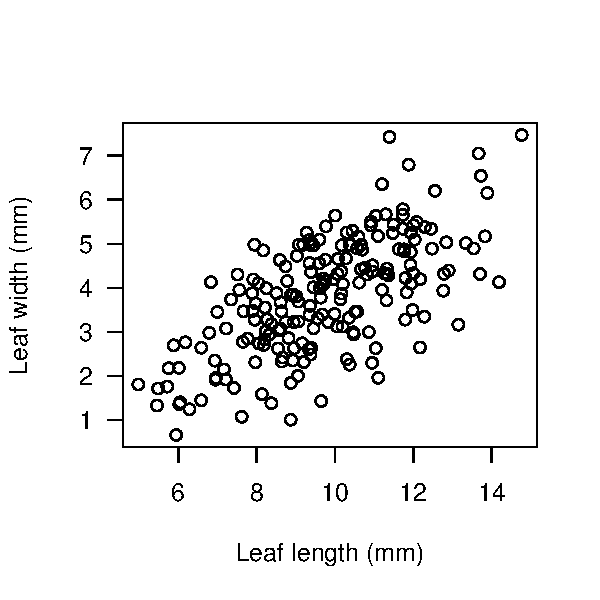
\includegraphics{Chapter2_LinReg_files/figure-latex/unnamed-chunk-10-1.pdf}

For a simple model like this, the expected attenuation bias (downward
bias) in the slope can be estimated by the reliability ratio

\(K = 1-\frac{\sigma_{me}}{\sigma_x}\)

where \(\sigma_{me}\) is the measurement error variance and \(\sigma_x\)
is the variance in the predictor \(x\). We can thus obtain a corrected
slope as

\(\beta'=\frac{\beta}{K}\)

Try to correct your estimated slopes in this way, and a produce a plot
showing both the estimated and the corrected slope connected by line
segments.

\begin{verbatim}
##  [1] 2.562152e-05 1.064084e-03 3.621491e-03 7.697843e-03 1.329314e-02
##  [6] 2.040738e-02 2.904057e-02 3.919270e-02 5.086378e-02 6.405380e-02
\end{verbatim}

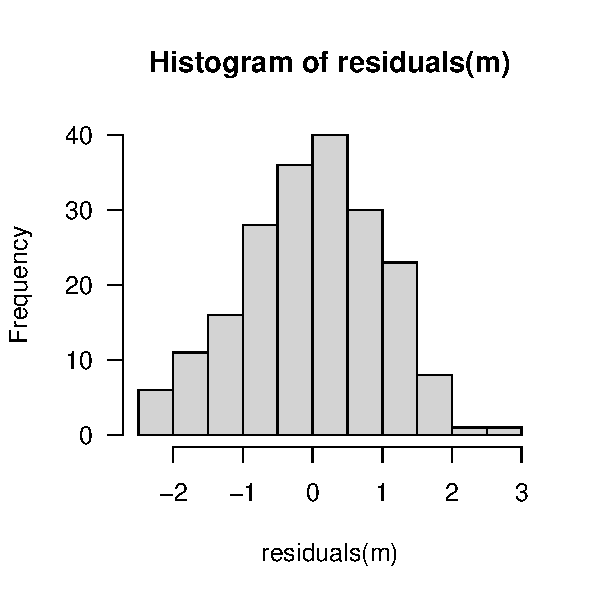
\includegraphics{Chapter2_LinReg_files/figure-latex/unnamed-chunk-11-1.pdf}

\hypertarget{exercise-fitting-a-linear-regression-to-real-data}{%
\subsubsection{Exercise: fitting a linear regression to real
data}\label{exercise-fitting-a-linear-regression-to-real-data}}

Choose any dataset you may have involving a continuous response variable
and an continuous predictor. Fit a simple linear regression, interpret
the results, produce a nice figure including the fitted regression line,
and write simple methods and results presenting the analysis and
results.

If you don't have any data, use the dataset \texttt{bird\_allometry} in
the datasets folder. This dataset contains body mass and brain mass for
males and females of different bird species. The scaling of brain size
(or other body parts) with body size is referred to as the study of
allometry, and you may want to read about these analyses before fitting
your models. As a hint, the scaling of parts of a body with body size is
expected to follow a power-law relationship on the form \(y = ax^b\),
which can be linearized through the logarithmic transformation
\(log(y) =log(a) + b \times log(x)\).

\begin{Shaded}
\begin{Highlighting}[]
\NormalTok{birds }\OtherTok{=} \FunctionTok{read.csv}\NormalTok{(}\StringTok{"datasets/allometry/bird\_allometry.csv"}\NormalTok{)}
\FunctionTok{head}\NormalTok{(birds)}
\end{Highlighting}
\end{Shaded}

\begin{verbatim}
##               Genus_Species Sex brain_mass body_mass
## 1        Accipiter_gentilis   f   7.686143 1049.1571
## 2        Accipiter_gentilis   m   7.618500  678.2833
## 3           Accipiter_nisus   f   3.112797  252.1263
## 4           Accipiter_nisus   m   2.637390  136.1441
## 5        Accipiter_striatus   f   5.700000  520.0000
## 6 Acridotheres_cristatellus   m   2.310000  122.3800
\end{verbatim}

\end{document}
